%% 
%% Copyright 2007-2020 Elsevier Ltd
%% 
%% This file is part of the 'Elsarticle Bundle'.
%% ---------------------------------------------
%% 
%% It may be distributed under the conditions of the LaTeX Project Public
%% License, either version 1.2 of this license or (at your option) any
%% later version.  The latest version of this license is in
%%    http://www.latex-project.org/lppl.txt
%% and version 1.2 or later is part of all distributions of LaTeX
%% version 1999/12/01 or later.
%% 
%% The list of all files belonging to the 'Elsarticle Bundle' is
%% given in the file `manifest.txt'.
%% 

%% Template article for Elsevier's document class `elsarticle'
%% with numbered style bibliographic references
%% SP 2008/03/01
%%
%% 
%%
%% $Id: elsarticle-template-num.tex 190 2020-11-23 11:12:32Z rishi $
%%
%%
\documentclass[preprint,12pt]{elsarticle}
%% Use the option review to obtain double line spacing
%% \documentclass[authoryear,preprint,review,12pt]{elsarticle}

%% Use the options 1p,twocolumn; 3p; 3p,twocolumn; 5p; or 5p,twocolumn
%% for a journal layout:
%% \documentclass[final,1p,times]{elsarticle}
%% \documentclass[final,1p,times,twocolumn]{elsarticle}
%% \documentclass[final,3p,times]{elsarticle}
%% \documentclass[final,3p,times,twocolumn]{elsarticle}
%% \documentclass[final,5p,times]{elsarticle}
%% \documentclass[final,5p,times,twocolumn]{elsarticle}

%% For including figures, graphicx.sty has been loaded in
%% elsarticle.cls. If you prefer to use the old commands
%% please give \usepackage{epsfig}

%% The amssymb package provides various useful mathematical symbols
\usepackage{amssymb}
\usepackage{relsize}
\usepackage{array}
\usepackage{caption}
\usepackage{subcaption}

\newcolumntype{L}[1]{>{\raggedright\let\newline\\\arraybackslash\hspace{0pt}}m{#1}}
\newcolumntype{C}[1]{>{\centering\let\newline\\\arraybackslash\hspace{0pt}}m{#1}}
\newcolumntype{R}[1]{>{\raggedleft\let\newline\\\arraybackslash\hspace{0pt}}m{#1}}

%% The amsthm package provides extended theorem environments
%% \usepackage{amsthm}

%% The lineno packages adds line numbers. Start line numbering with
%% \begin{linenumbers}, end it with \end{linenumbers}. Or switch it on
%% for the whole article with \linenumbers.
%% \usepackage{lineno}

\journal{Neural Networks}

\begin{document}

\begin{frontmatter}

%% Title, authors and addresses

%% use the tnoteref command within \title for footnotes;
%% use the tnotetext command for theassociated footnote;
%% use the fnref command within \author or \address for footnotes;
%% use the fntext command for theassociated footnote;
%% use the corref command within \author for corresponding author footnotes;
%% use the cortext command for theassociated footnote;
%% use the ead command for the email address,
%% and the form \ead[url] for the home page:
%% \title{Title\tnoteref{label1}}
%% \tnotetext[label1]{}
%% \author{Name\corref{cor1}\fnref{label2}}
%% \ead{email address}
%% \ead[url]{home page}
%% \fntext[label2]{}
%% \cortext[cor1]{}
%% \affiliation{organization={},
%%             addressline={},
%%             city={},
%%             postcode={},
%%             state={},
%%             country={}}
%% \fntext[label3]{}

\title{Signed Saliency Maps}

%% use optional labels to link authors explicitly to addresses:
%% \author[label1,label2]{}
%% \affiliation[label1]{organization={},
%%             addressline={},
%%             city={},
%%             postcode={},
%%             state={},
%%             country={}}
%%
%% \affiliation[label2]{organization={},
%%             addressline={},
%%             city={},
%%             postcode={},
%%             state={},
%%             country={}}

\author[inst1]{Oscar Llorente}

\affiliation[inst1]{organization={BMAS SA NDO SW R\&D Unit B, Ericsson},%Department and Organization
            addressline={Retama Ed 1 Torre Suecia}, 
            city={Madrid},
            postcode={28045}, 
            state={Madrid},
            country={Spain}}

\author[inst2]{Jaime Boal}
\author[inst2]{Eugenio F. Sánchez-Úbeda}

\affiliation[inst2]{organization={Institute for Research in Technology~(IIT), ICAI School of Engineering, Comillas Pontifical University},%Department and Organization
            addressline={Santa Cruz de Marcenado, 26}, 
            city={Madrid},
            postcode={28015}, 
            state={Madrid},
            country={Spain}}

\begin{abstract}
%% Text of abstract
Lorem ipsum dolor sit amet, consectetur adipiscing elit, sed do eiusmod tempor incididunt ut labore et dolore magna aliqua. Ut enim ad minim veniam, quis nostrud exercitation ullamco laboris nisi ut aliquip ex ea commodo consequat. Duis aute irure dolor in reprehenderit in voluptate velit esse cillum dolore eu fugiat nulla pariatur. Excepteur sint occaecat cupidatat non proident, sunt in culpa qui officia deserunt mollit anim id est laborum.
\end{abstract}

%%Graphical abstract
\begin{graphicalabstract}
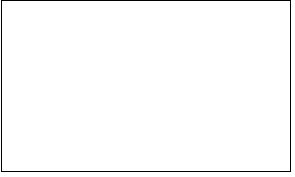
\includegraphics{grabs}
\end{graphicalabstract}

%%Research highlights
\begin{highlights}
\item Research highlight 1
\item Research highlight 2
\end{highlights}

\begin{keyword}
%% keywords here, in the form: keyword \sep keyword
keyword one \sep keyword two
%% PACS codes here, in the form: \PACS code \sep code
\PACS 0000 \sep 1111
%% MSC codes here, in the form: \MSC code \sep code
%% or \MSC[2008] code \sep code (2000 is the default)
\MSC 0000 \sep 1111
\end{keyword}

\end{frontmatter}

%% \linenumbers

%% main text
\section{Introduction}
\label{sec:introduction}
Since the introduction of AlexNet~\cite{krizhevskyImageNetClassificationDeep2012} in the ImageNet~\cite{ImageNet} competition there has been a revolution in the Computer Vision field, where almost in any problem deep learning architectures are the considered the state of the art. However, this type of technology has a big drawback, specially if it is used in sensitive domains, as medicine or autonomous vehicles, its explainability. Due to the high number of parameters (billions) and the complexity of these techniques, it is difficult to explain how a neural network make a certain prediction. To solve this problem, there are two main lines of research:

\begin{itemize}
    \item Building more interpretable models.
    \item Developing techniques to explain the state of the art techniques.
\end{itemize}

There have been attempts to construct these interpretable models for the sensitive domains as in~\cite{singhThinkPositiveInterpretable2022}. However, there are also many other techniques used for Computer Vision problems that offer great results and are not easy to explain, as the classical Convolutional Neural Networks (CNNs)~\cite{lecunConvolutionalNetworksImages}. To explaining these other models  several techniques have been developed during the last years. One of the most used types are Saliency Maps.

Saliency Maps were introduced first in~\cite{simonyanDeepConvolutionalNetworks2014a} to explain the classification of a neural network based on its derivatives. This type of methods are commonly tested in a multi-class classification problem that can be defined as the following:

\begin{equation}
    \label{eq: cnn output}
    class(I) = argmax_{c \in C}S_c(I),
\end{equation}

\noindent
being $I$ the input image, $C$ the set of all possible classes and $S_c$ the classification score. Then, the original Saliency Map method is expressed as:

\begin{equation}
    \label{eq: saliency map}
    M_c(I) = max_{channel}\bigg \{ \bigg |\frac{\partial S_c}{\partial I} \bigg | \bigg \}.
\end{equation}

\noindent
According to~\cite{simonyanDeepConvolutionalNetworks2014a}, the brightest points in a Saliency Map, i.e., the derivatives with a higher absolute value, are the points that, with a minimum change, affect the class score the most. Then, to derive a single value per pixel, the maximum function over the three pixels is computed. Even though this decision can seem arbitrary, this is the convention that has been followed in every paper about Saliency Maps.

However, the original Saliency Maps are very noisy. Therefore, in the following years many variations were suggested to try to improve this visualization and make this noise disappear, as in \cite{springenbergStrivingSimplicityAll2015}, \cite{sundararajanAxiomaticAttributionDeep2017} or \cite{shrikumarNotJustBlack2017}. By this, sharper visualizations were achieved, being these ones more similar to the object in the image and reducing the noise. Unfortunately, in~\cite{adebayoSanityChecksSaliency2018} it was proved that some of these techniques were not showing information about what the neural network has learned, but features from the image, as an edge detector. 

Nevertheless, there is no need of these techniques that improve the visualizations by projecting the image information: more knowledge can be unlocked from the gradients of the neural network without further modifications. First, as far as we know, the sign of the gradients has not been studied in any paper. This sign can have a meaning and a significant impact in the neural network behavior that researchers are trying to understand. Moreover, the type of problem being studied is a multi-class classification problem, and a visualization that tries to explain that, should take into account all these classes and not only the one that is being predicted. In other words, the magnitude of the gradients can have different meaning if it is greater or smaller than the gradients for other classes. 

\section{The Sign in Saliency Maps}
\label{sec:the sign in saliency maps}
As pointed out in the last section, there is not any research about the meaning or impact of the sign in Saliency Maps. The only article that discuss briefly this aspect is~\cite{smilkovSmoothGradRemovingNoise}. In this paper it was explained that the raw value of gradients (without absolute value) is commonly used for MNIST dataset~\cite{MNISTHandwrittenDigit} but not in other datasets as ImageNet. The reason for this is that in the former it produces clearer pictures and in the latter is the opposite. 

However, by taking the absolute value of all the pixels in the Saliency Map, information can be lost. It is not only valuable knowing which pixels are important but also their meaning. For example, it would be significant, for the explainability field, having a technique that can indicate which zones of the image should be brighter to improve the classification and which ones should be darker. This is in fact the information that the sign can provide. Moreover, if both information are combined in the same image without any distinctions between them, they can produce worse explanations. It can seem as if the model is not able to distinguish between zones that should be brighter and others that should be brighter, as for example an object in front of a darker background. Based on this, two sets of pixels can be distinguished in the image:

\begin{itemize}
    \item Pixels that by increasing their value the classification of the model improves\footnote{It is important to note that improving the model classification means that the logit of the predicted class increases. } since they have a positive value in the Saliency Map (positive gradient).
    \item Pixels that by decreasing their value the classification of the model improves since they have a negative value in the Saliency Map (negative gradient).
\end{itemize}

Regarding the reason for not using the raw values exposed in~\cite{smilkovSmoothGradRemovingNoise}, it can be due to a high number of 0 values in the Saliency Map, since when normalized with positives and negatives these pixels will be shining at a medium intensity. To solve this, in this paper the visualization in different images is proposed, having the following new techniques:

\begin{itemize}
    \item Positive Saliency Maps:
    
    \begin{equation}
        \label{eq: positive saliency map}
        M_c(I) = max_{channel}\bigg \{ ReLU \bigg (\frac{\partial S_c}{\partial I} \bigg ) \bigg \}.
    \end{equation}

    \item Negative Saliency Maps:
    
    \begin{equation}
        \label{eq: negative saliency map}
        M_c(I) = max_{channel}\bigg \{ ReLU \bigg (-\frac{\partial S_c}{\partial I} \bigg ) \bigg \}
    \end{equation}

\end{itemize}

By separating them before taking the absolute value the information about what the pixels mean is not lost. 

\section{Multi-class Saliency Maps}
\label{sec:multi-class saliency map}
As it was mentioned in Section~\ref{sec:introduction}, the problem being studied is a multi-class classification problem. However, currently all Saliency Map techniques used the predicted class to compute the derivatives. That does not take into account the information about other classes that the model is predicting. In other words, there can be another gradient for other class with a higher value than for the predicted class and the current techniques cannot show that to the user. The reason for this is that, if the absolute value of all gradients is taken, there cannot be any comparison with the gradients of other classes, since there is no information anymore that can indicate what means that a gradient is higher or lower than another.

However, going further in the analysis started in the last section about the sign allows to compare the gradients of the predicted class and the other ones. In fact, it improves the previous definitions about the different sets of pixels identified in the last section:

\begin{itemize}
    \item Pixels that by increasing their value the classification of the model improves\footnote{Since now the other classes are taken into account, the definition of improving the classification is that the difference of the logit of the predicted class and the other logits is greater.} are not always the positive ones. Since now other classes are taken into account, only the pixels that have a higher gradient for the predicted class that for any other class, will improve the classification if their value is increased.
    \item Analogously, the pixels that by decreasing their value improve the classification are only the ones that have a lower gradient for the predicted class than for any other class.
\end{itemize}

Therefore, by comparing the Saliency Maps for the different classes the information about the two sets mentioned before can be extracted. Two new techniques are proposed to represent this:

\begin{itemize}
    \item Active Saliency Map (increasing them improves the classification):
    
    \begin{equation}
        \label{eq: active saliency map}
        \hat{M}_c(I) = max_{channel} \bigg \{ M_c \mathlarger{\mathlarger{\prod}}_{q \in (C-c)}M_c > \frac{\partial S_q}{\partial I} \bigg \},
    \end{equation}

    being $M_c$ the Saliency Map (original technique) for the predicted class $c$.

    \item Inactive Saliency Map (decreasing them improves the classification):
    
    \begin{equation}
        \label{eq: inactive saliency map}
        \hat{M}_c(I) = max_{channel} \bigg \{ M_c \mathlarger{\mathlarger{\prod}}_{q \in (C-c)}M_c < \frac{\partial S_q}{\partial I} \bigg \}.
    \end{equation}

\end{itemize}

\section{Experiments}
\label{sec:experiments}
In this section the new proposed techniques will be evaluated qualitatively and quantitatively. With this purpose, a certain methodology was followed. First, two datasets are used to study the new methods, Cifar10~\cite{CIFAR10CIFAR100Datasets} and Imagenette~\cite{Imagenette2022}. The first one is a commonly used dataset for image classification and also for explainability. The second one is a subset of 10 classes of Imagenet. It is used this subset instead of the original Imagenet due to computing restrictions of hardware. Then, two models are trained for each dataset. The first is a CNN model based in a max-pooling several layers for CNNs, and average-pooling and a final linear layer. The second one is the classical Resnet18~\cite{heDeepResidualLearning2016}. They were all trained with a learning rate of $0.001$ and the AdamW optimizer for 50 epochs. The results of the test set are the following:

\begin{table}[h!]
    \begin{center}
        \begin{tabular}{|L{0.2\linewidth}|C{0.2\linewidth}|C{0.2\linewidth}|}
            \hline
            \textbf{} & \textbf{Cifar10} & \textbf{Imagenette}\\ \hline
            \textbf{Basic CNN model} & 0.6307 & 0.6205 \\ \hline
            \textbf{Resnet18} & 0.7569 & 0.8357 \\ \hline
        \end{tabular}
        \caption{Training results}
        \label{tab: training results}
    \end{center}
\end{table}

\subsection{Qualitative Evaluation}

\begin{figure}
    \centering
    \begin{subfigure}{0.14\linewidth}
        \centering
        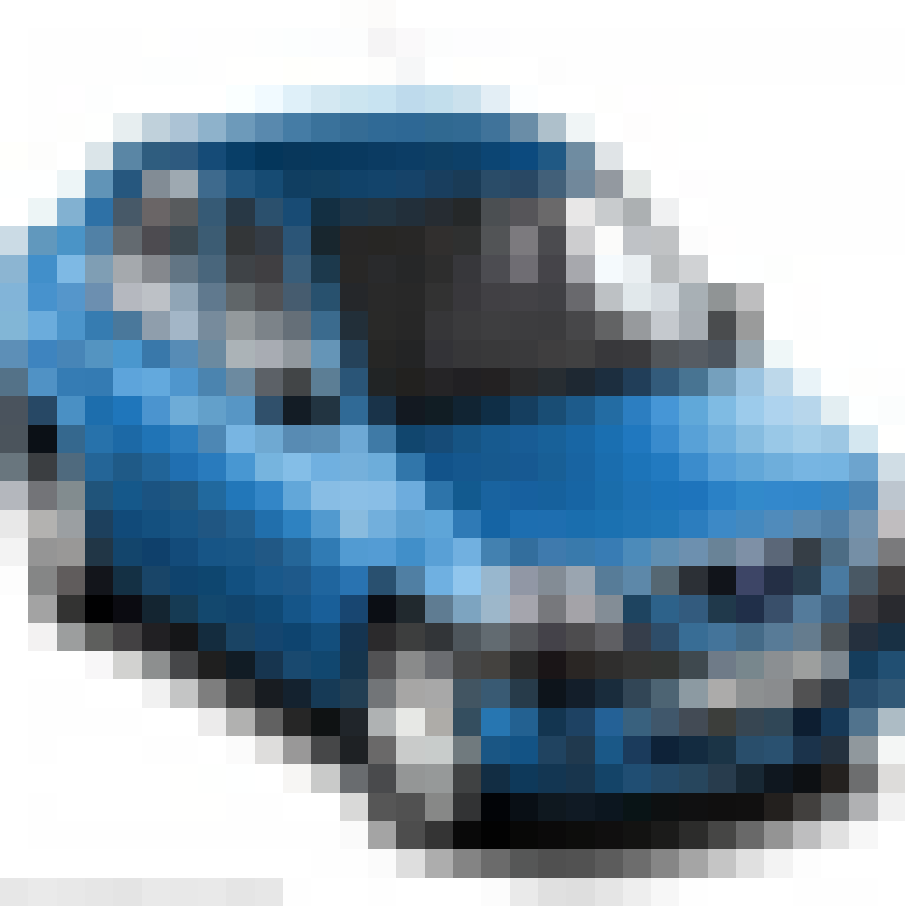
\includegraphics[width=\linewidth]{../visualizations/examples/cifar10/cnn/images/1.png}
        \caption{image}
    \end{subfigure}
    \hfill
    \begin{subfigure}{0.14\linewidth}
        \centering
        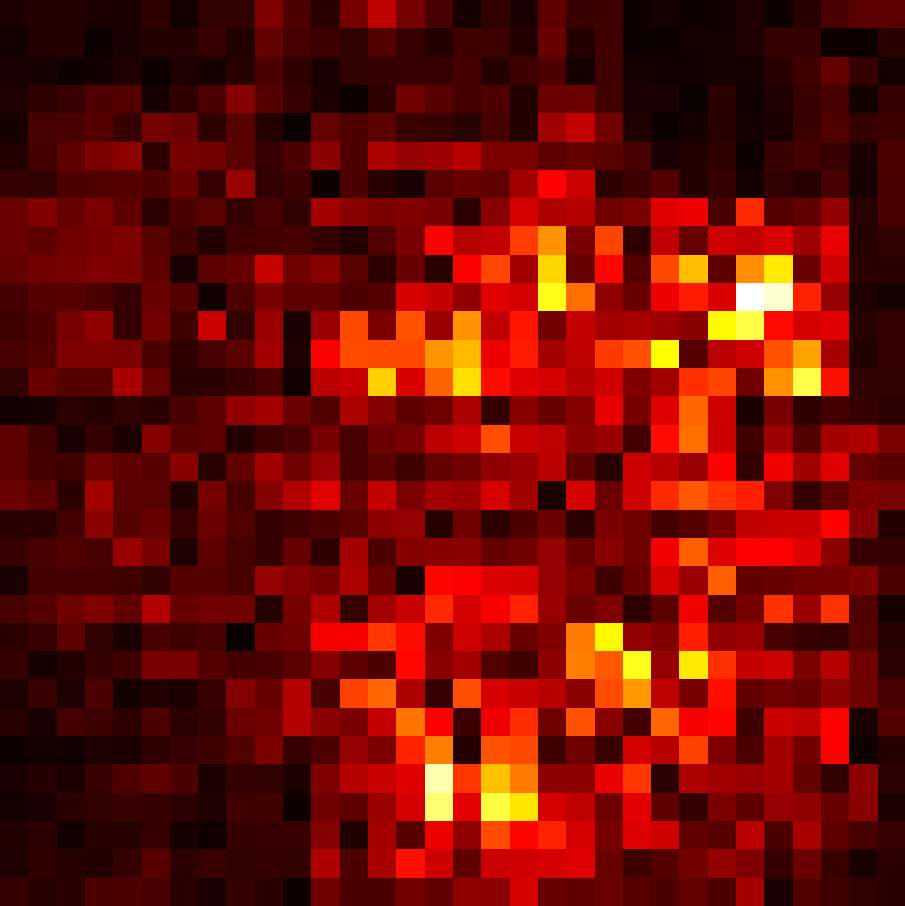
\includegraphics[width=\linewidth]{../visualizations/examples/cifar10/cnn/saliency_map/1.png}
        \caption{original}
    \end{subfigure}
    \hfill
    \begin{subfigure}{0.14\textwidth}
        \centering
        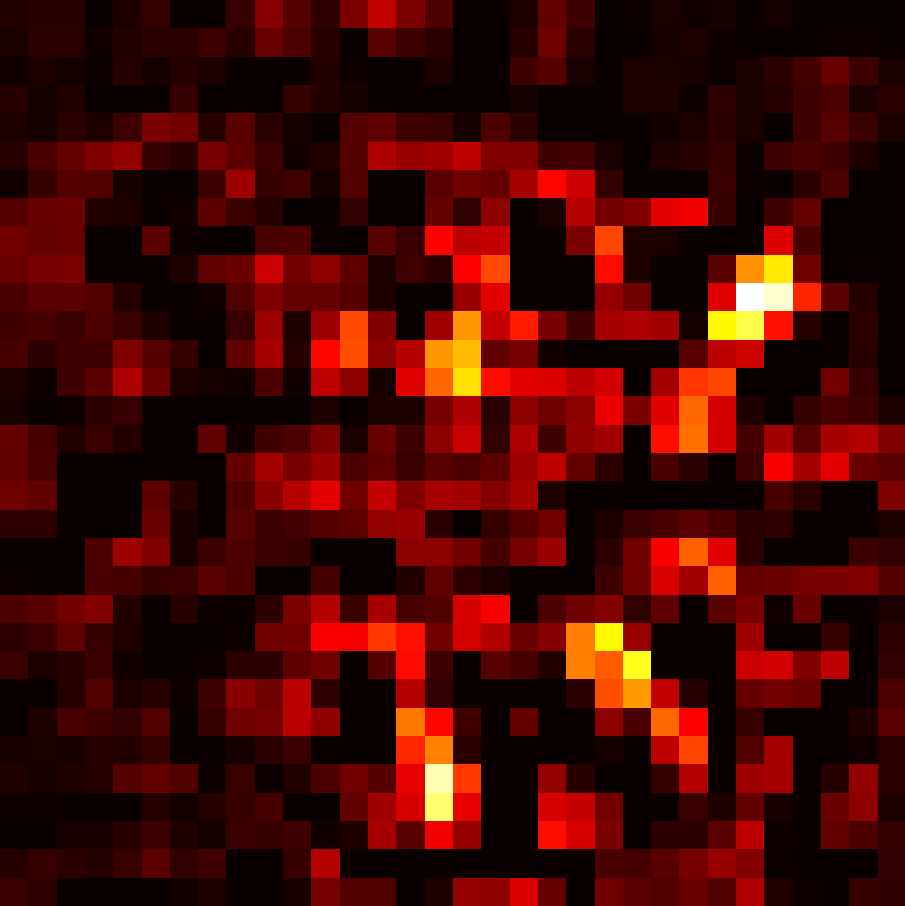
\includegraphics[width=\linewidth]{../visualizations/examples/cifar10/cnn/positive_saliency_map/1.png}
        \caption{positive}
    \end{subfigure}
    \hfill
    \begin{subfigure}{0.14\textwidth}
        \centering
        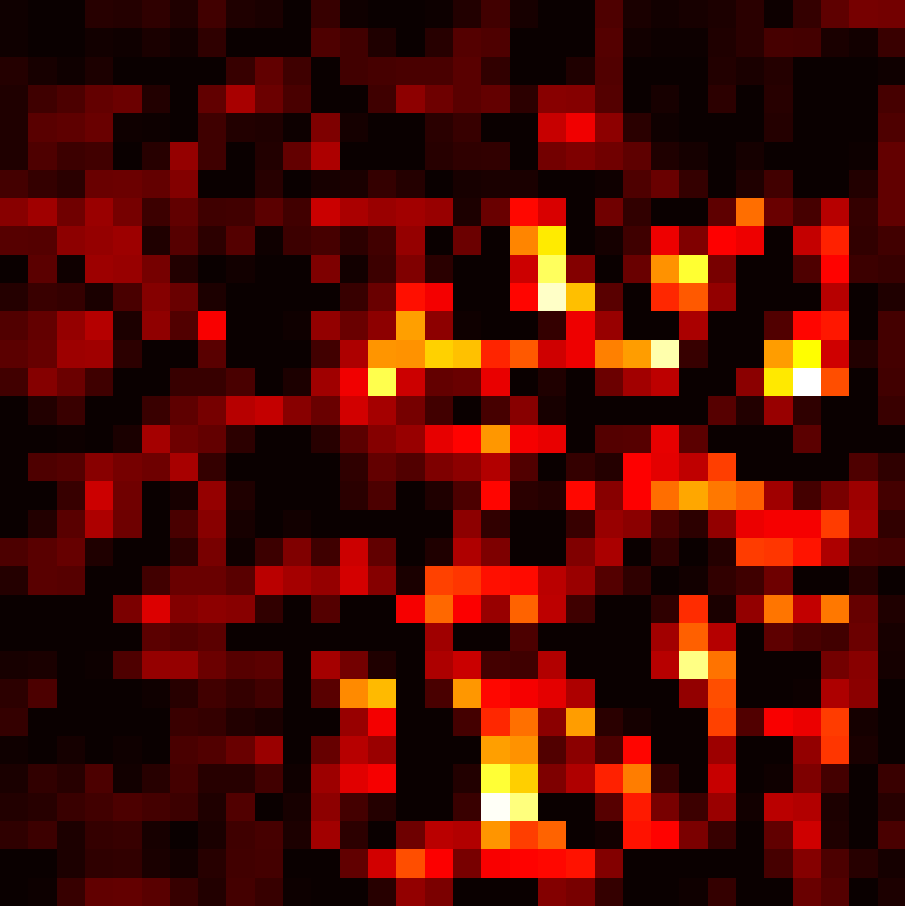
\includegraphics[width=\linewidth]{../visualizations/examples/cifar10/cnn/negative_saliency_map/1.png}
        \caption{negative}
    \end{subfigure}
    \hfill
    \begin{subfigure}{0.14\textwidth}
        \centering
        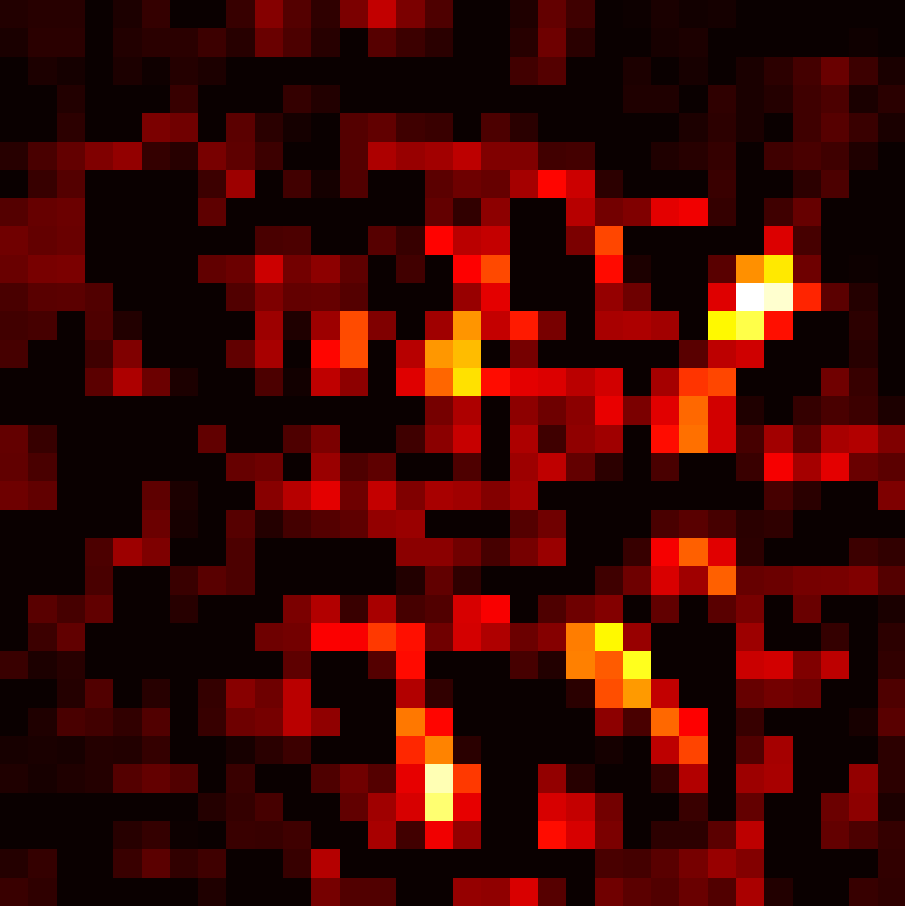
\includegraphics[width=\linewidth]{../visualizations/examples/cifar10/cnn/active_saliency_map/1.png}
        \caption{active}
    \end{subfigure}
    \hfill
    \begin{subfigure}{0.14\textwidth}
        \centering
        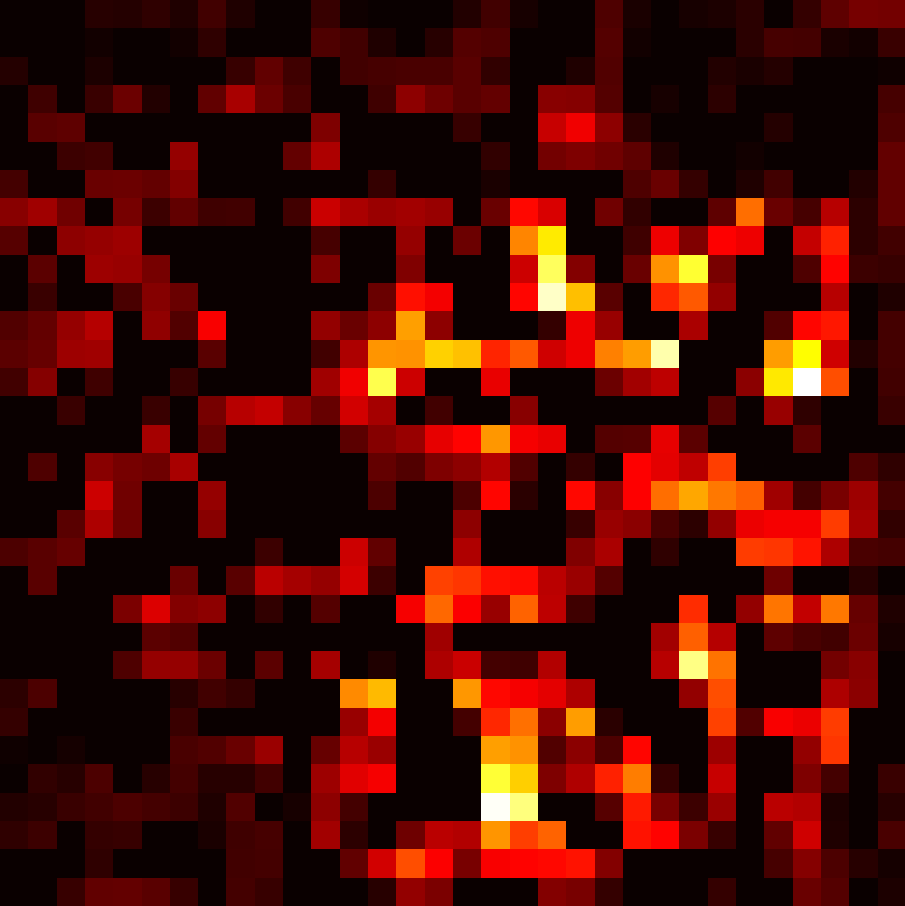
\includegraphics[width=\linewidth]{../visualizations/examples/cifar10/cnn/inactive_saliency_map/1.png}
        \caption{inactive}
    \end{subfigure}
    \begin{subfigure}{0.14\linewidth}
        \centering
        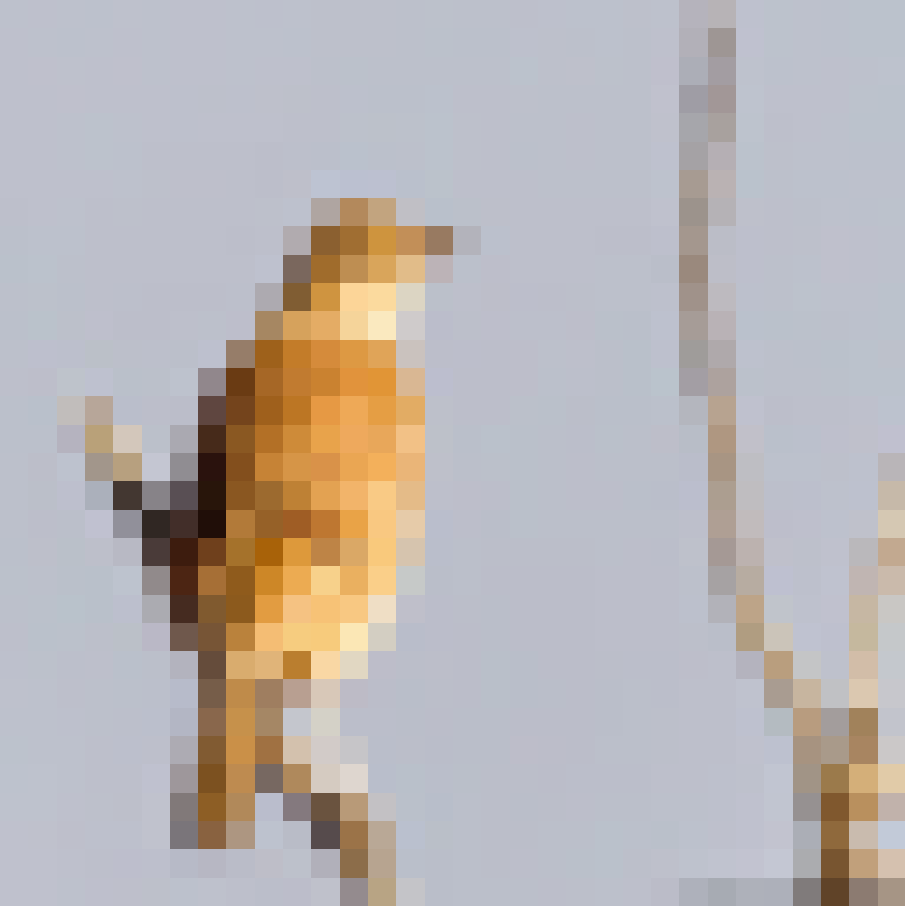
\includegraphics[width=\linewidth]{../visualizations/examples/cifar10/cnn/images/2.png}
        \caption{image}
    \end{subfigure}
    \hfill
    \begin{subfigure}{0.14\linewidth}
        \centering
        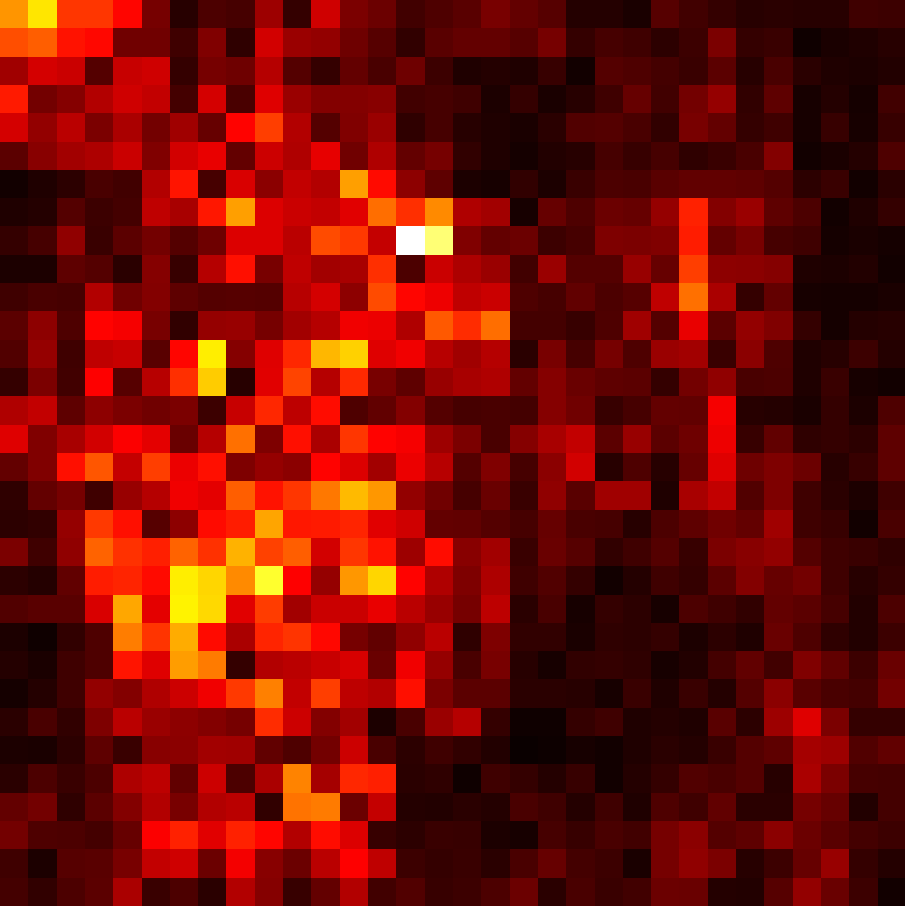
\includegraphics[width=\linewidth]{../visualizations/examples/cifar10/cnn/saliency_map/2.png}
        \caption{original}
    \end{subfigure}
    \hfill
    \begin{subfigure}{0.14\textwidth}
        \centering
        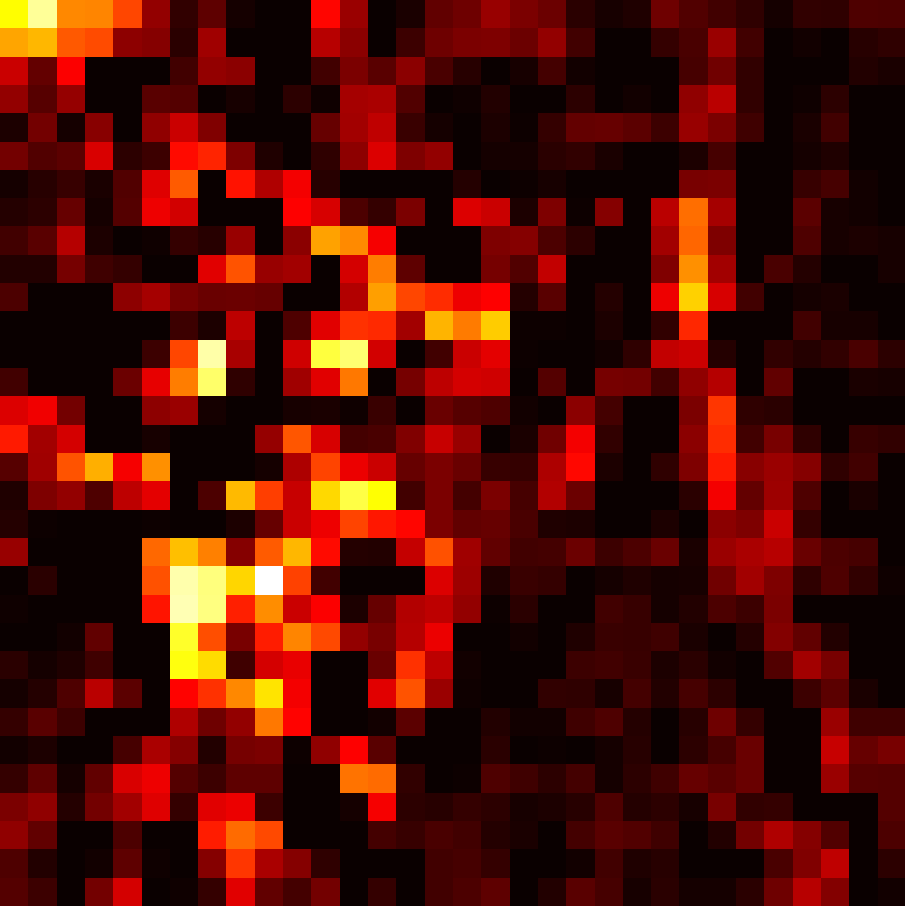
\includegraphics[width=\linewidth]{../visualizations/examples/cifar10/cnn/positive_saliency_map/2.png}
        \caption{positive}
    \end{subfigure}
    \hfill
    \begin{subfigure}{0.14\textwidth}
        \centering
        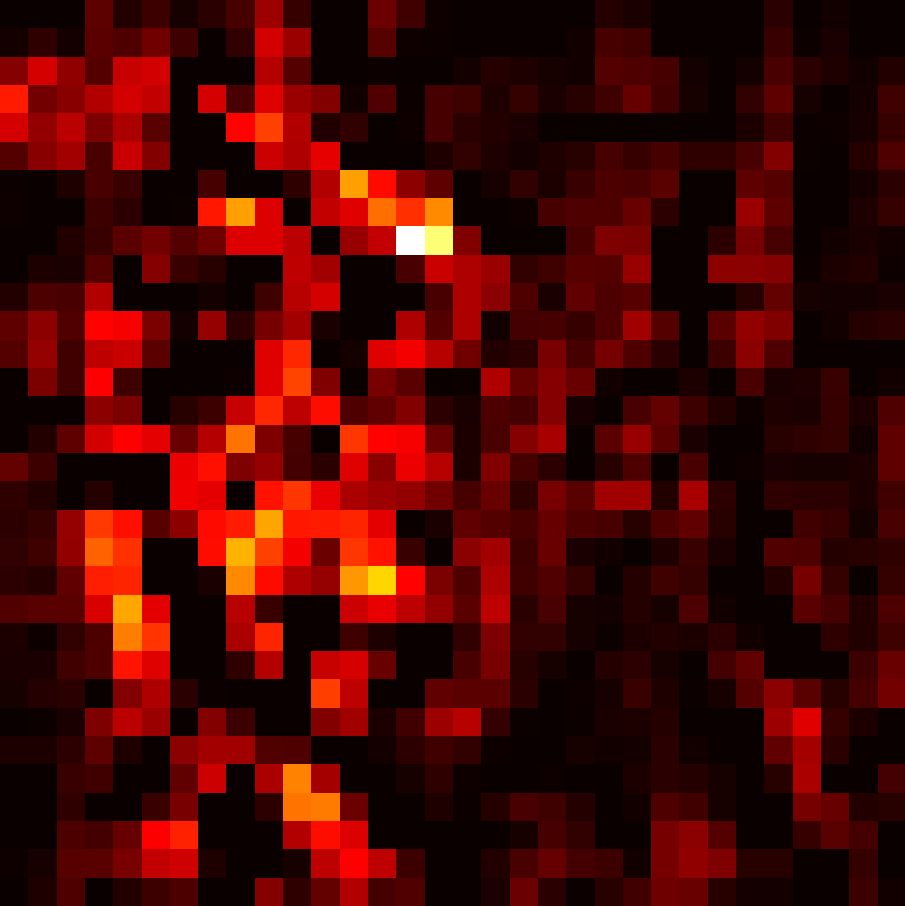
\includegraphics[width=\linewidth]{../visualizations/examples/cifar10/cnn/negative_saliency_map/2.png}
        \caption{negative}
    \end{subfigure}
    \hfill
    \begin{subfigure}{0.14\textwidth}
        \centering
        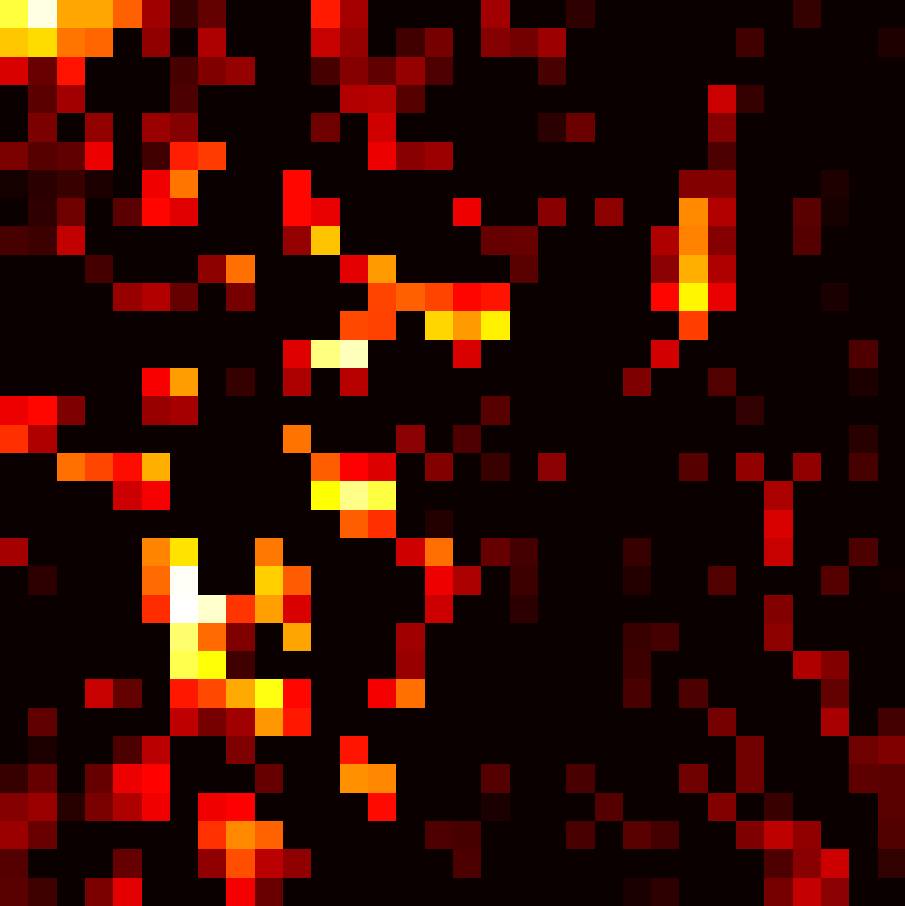
\includegraphics[width=\linewidth]{../visualizations/examples/cifar10/cnn/active_saliency_map/2.png}
        \caption{active}
    \end{subfigure}
    \hfill
    \begin{subfigure}{0.14\textwidth}
        \centering
        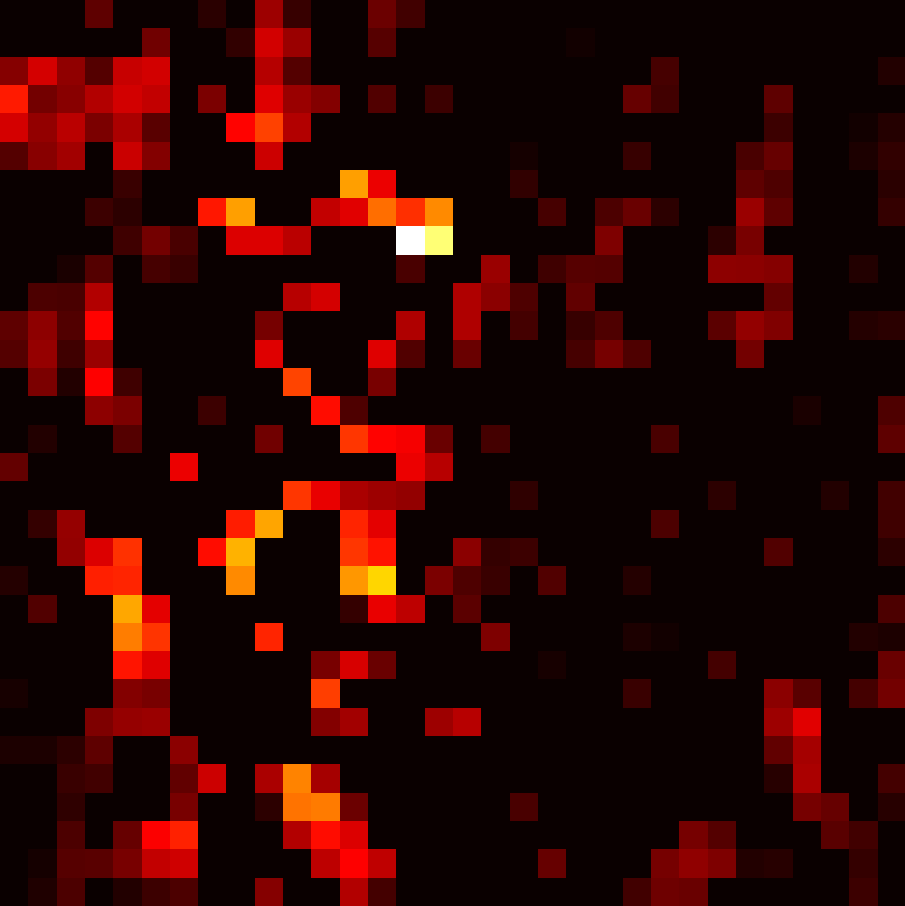
\includegraphics[width=\linewidth]{../visualizations/examples/cifar10/cnn/inactive_saliency_map/2.png}
        \caption{inactive}
    \end{subfigure}
    \caption{Comparison Saliency Maps CNN Cifar10}
    \label{fig: comparison saliency maps cnn cifar10}
\end{figure}

\begin{figure}
    \centering
    \begin{subfigure}{0.14\linewidth}
        \centering
        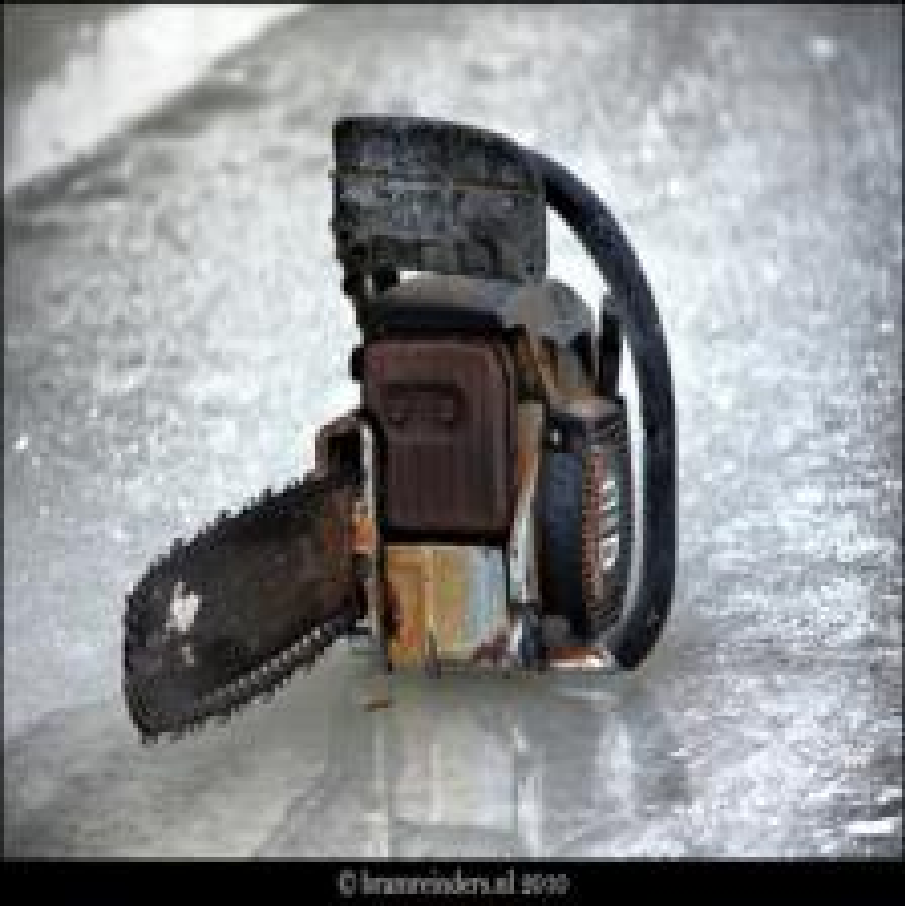
\includegraphics[width=\linewidth]{../visualizations/examples/imagenette/resnet18/images/0.png}
        \caption{image}
    \end{subfigure}
    \hfill
    \begin{subfigure}{0.14\linewidth}
        \centering
        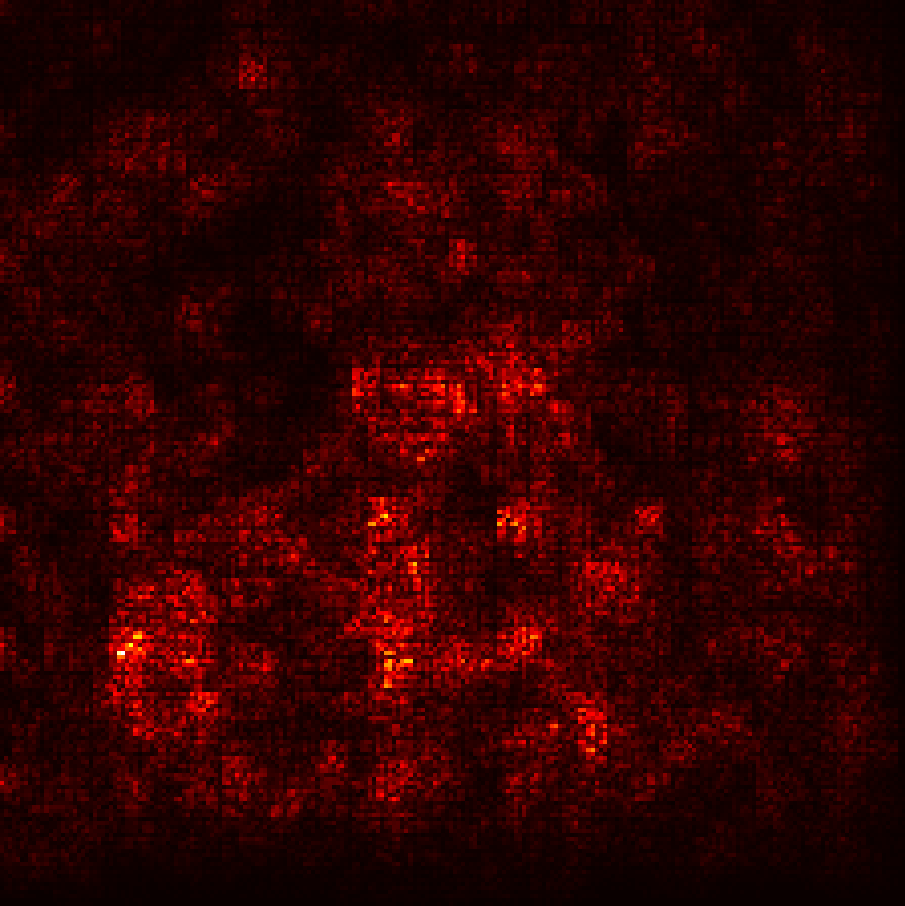
\includegraphics[width=\linewidth]{../visualizations/examples/imagenette/resnet18/saliency_map/0.png}
        \caption{original}
    \end{subfigure}
    \hfill
    \begin{subfigure}{0.14\textwidth}
        \centering
        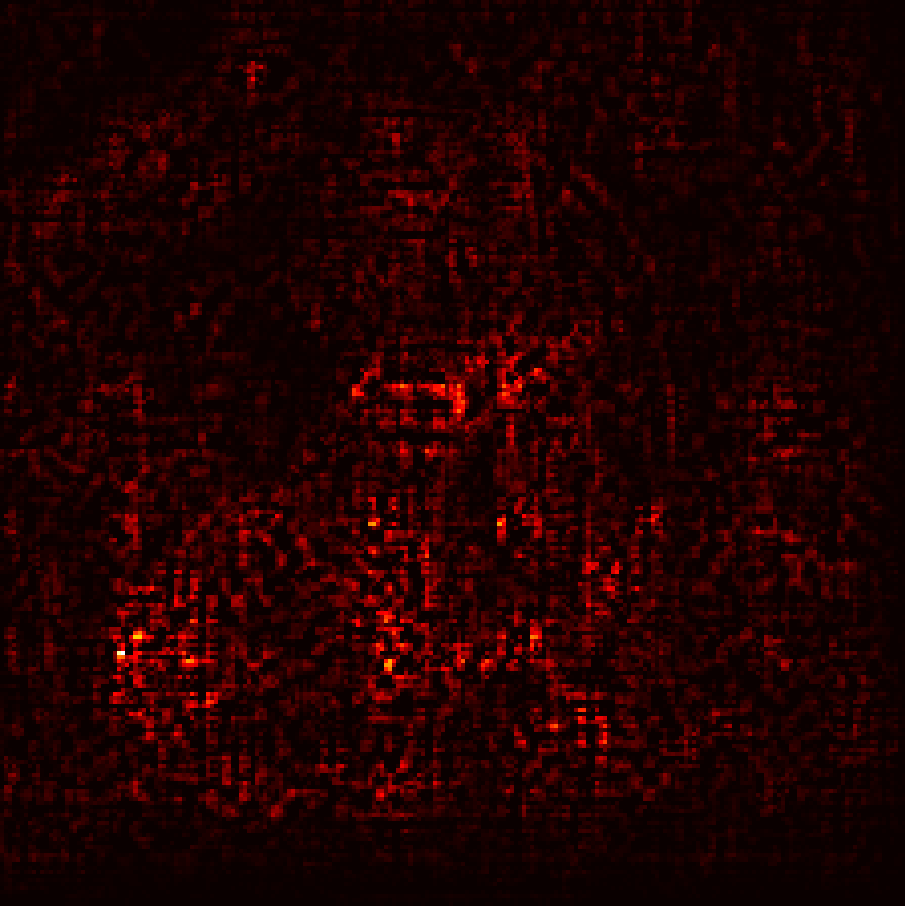
\includegraphics[width=\linewidth]{../visualizations/examples/imagenette/resnet18/positive_saliency_map/0.png}
        \caption{positive}
    \end{subfigure}
    \hfill
    \begin{subfigure}{0.14\textwidth}
        \centering
        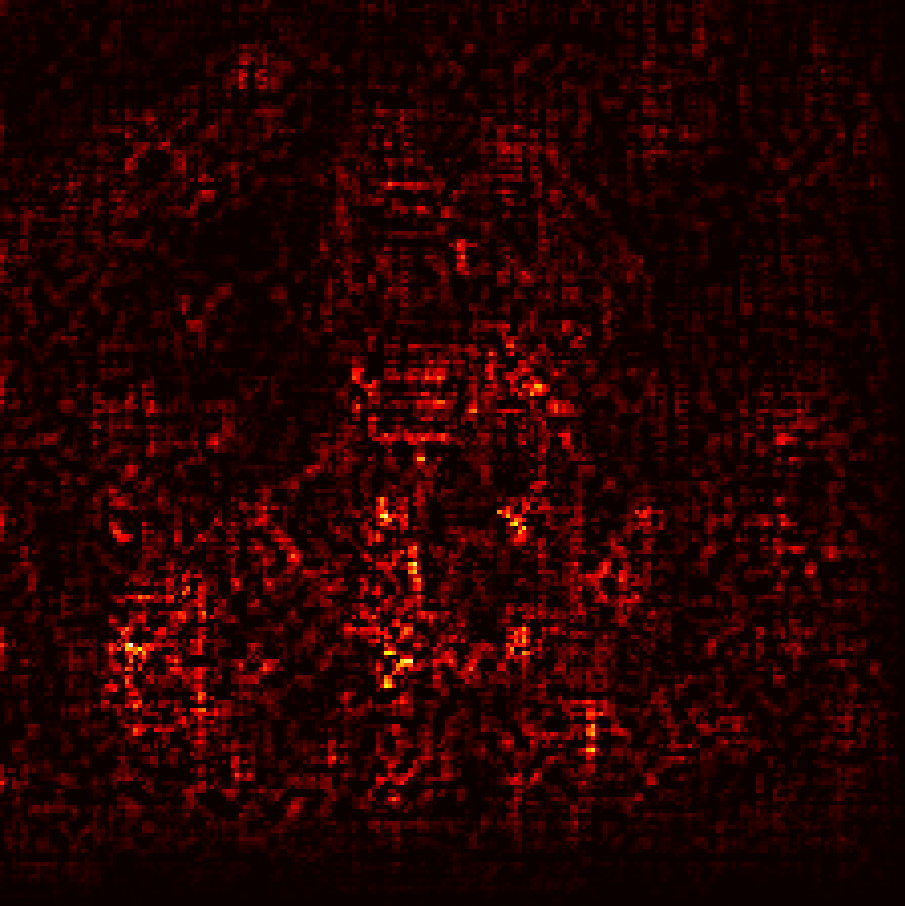
\includegraphics[width=\linewidth]{../visualizations/examples/imagenette/resnet18/negative_saliency_map/0.png}
        \caption{negative}
    \end{subfigure}
    \hfill
    \begin{subfigure}{0.14\textwidth}
        \centering
        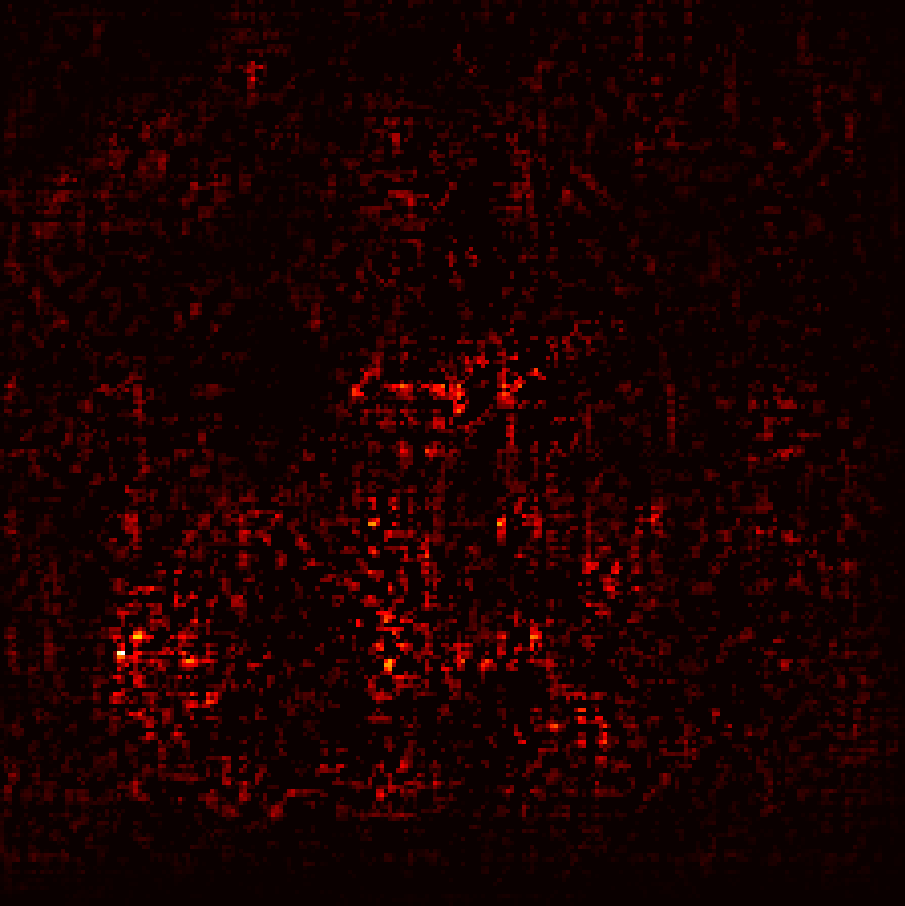
\includegraphics[width=\linewidth]{../visualizations/examples/imagenette/resnet18/active_saliency_map/0.png}
        \caption{active}
    \end{subfigure}
    \hfill
    \begin{subfigure}{0.14\textwidth}
        \centering
        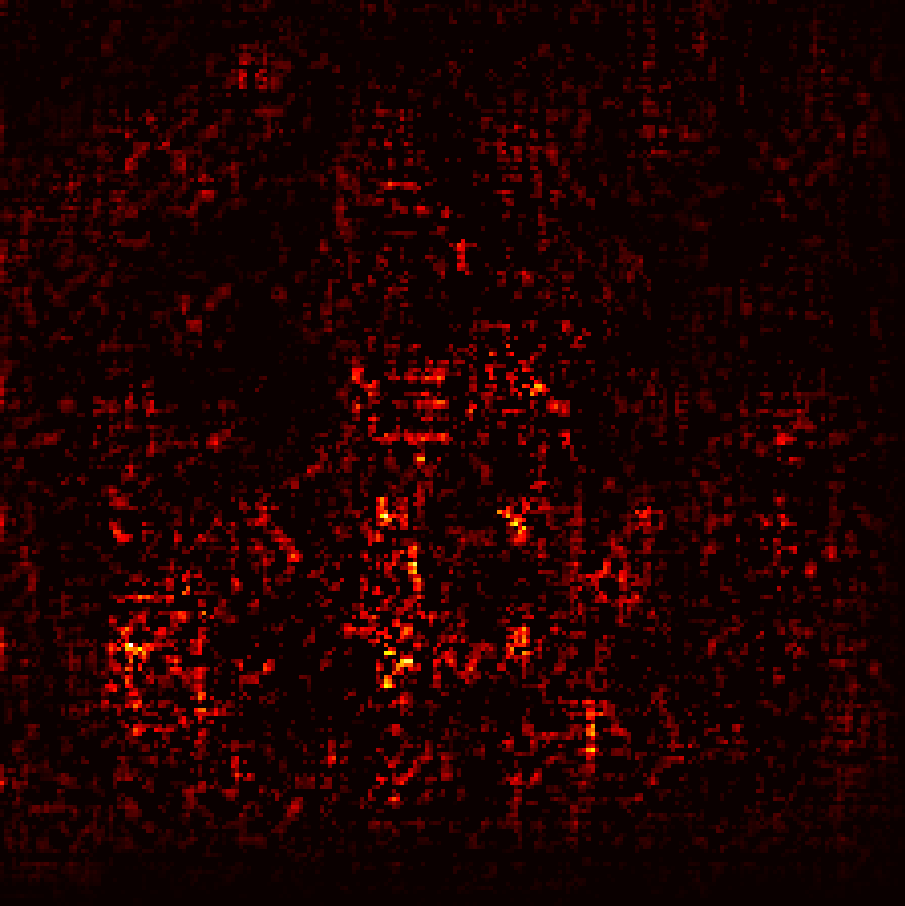
\includegraphics[width=\linewidth]{../visualizations/examples/imagenette/resnet18/inactive_saliency_map/0.png}
        \caption{inactive}
    \end{subfigure}\\
    \begin{subfigure}{0.14\linewidth}
        \centering
        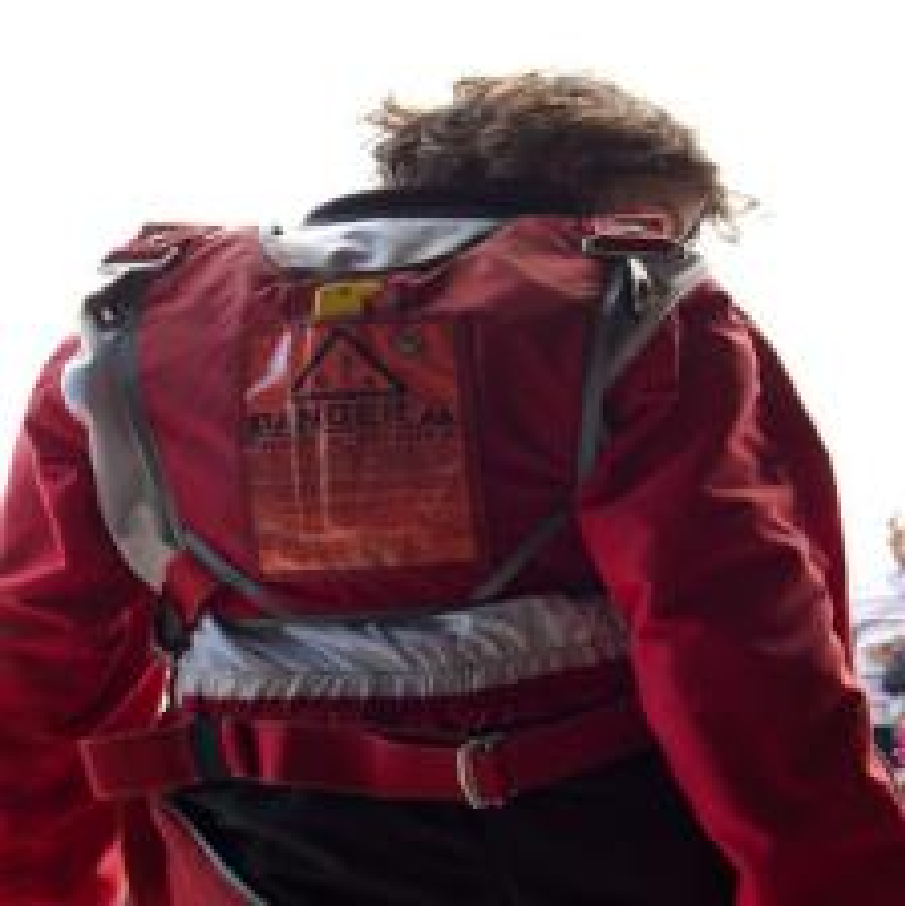
\includegraphics[width=\linewidth]{../visualizations/examples/imagenette/resnet18/images/8.png}
        \caption{image}
    \end{subfigure}
    \hfill
    \begin{subfigure}{0.14\linewidth}
        \centering
        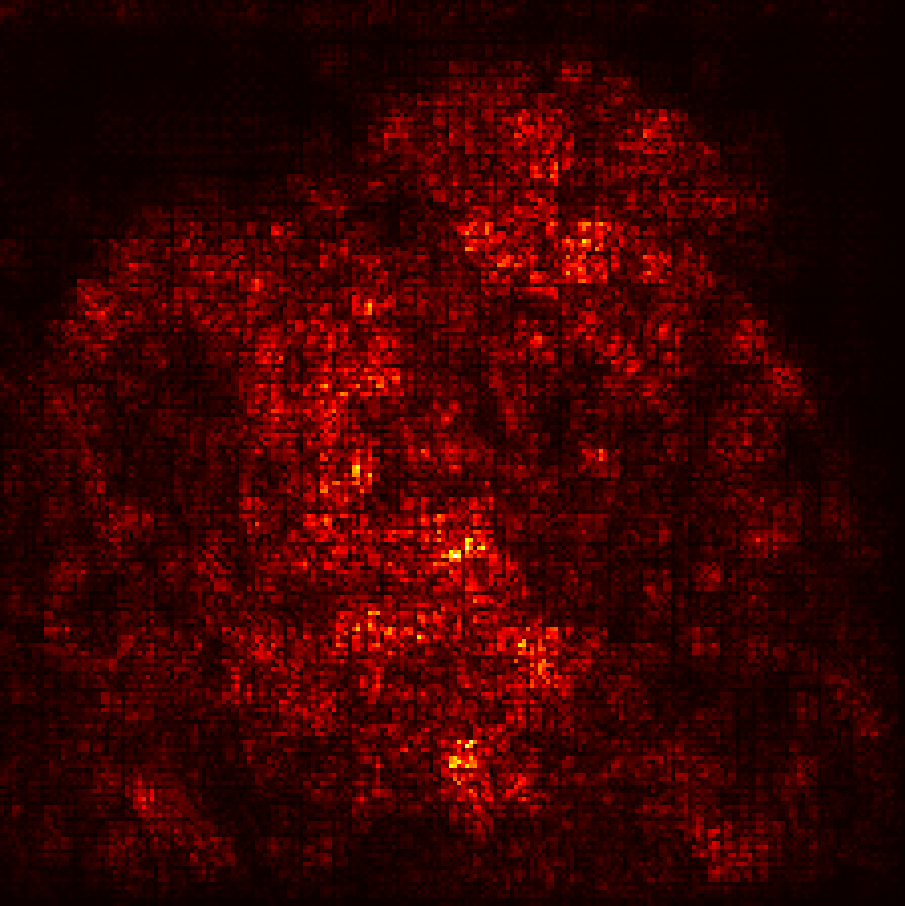
\includegraphics[width=\linewidth]{../visualizations/examples/imagenette/resnet18/saliency_map/8.png}
        \caption{original}
    \end{subfigure}
    \hfill
    \begin{subfigure}{0.14\textwidth}
        \centering
        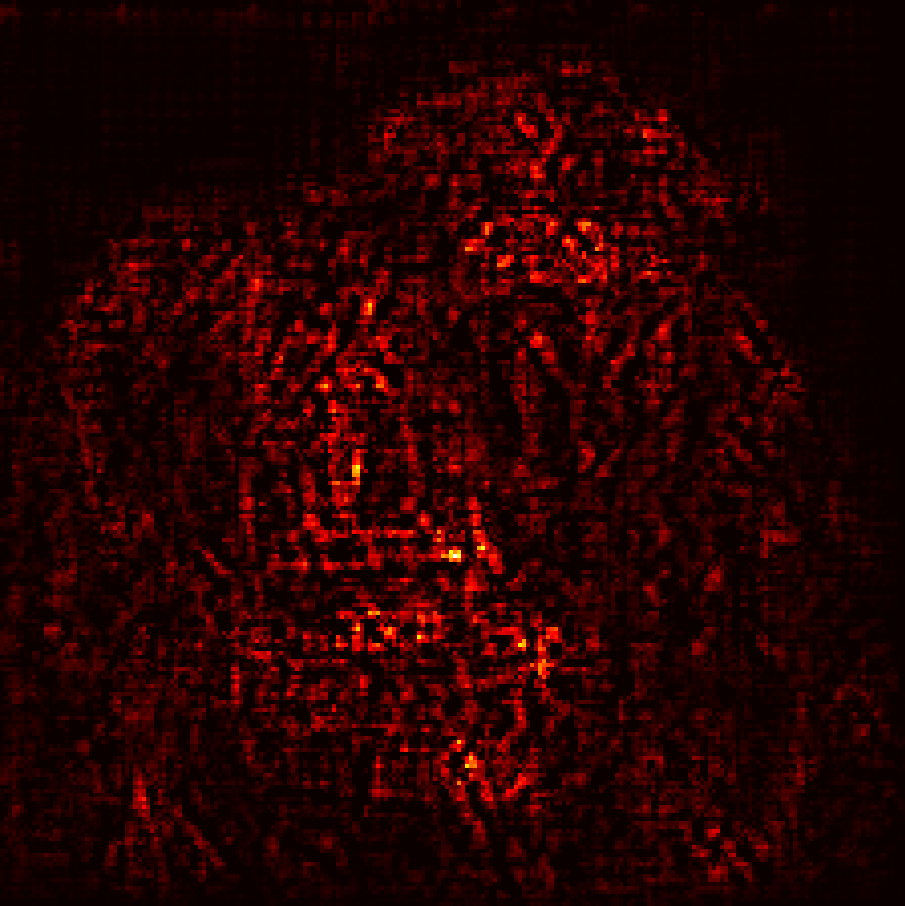
\includegraphics[width=\linewidth]{../visualizations/examples/imagenette/resnet18/positive_saliency_map/8.png}
        \caption{positive}
    \end{subfigure}
    \hfill
    \begin{subfigure}{0.14\textwidth}
        \centering
        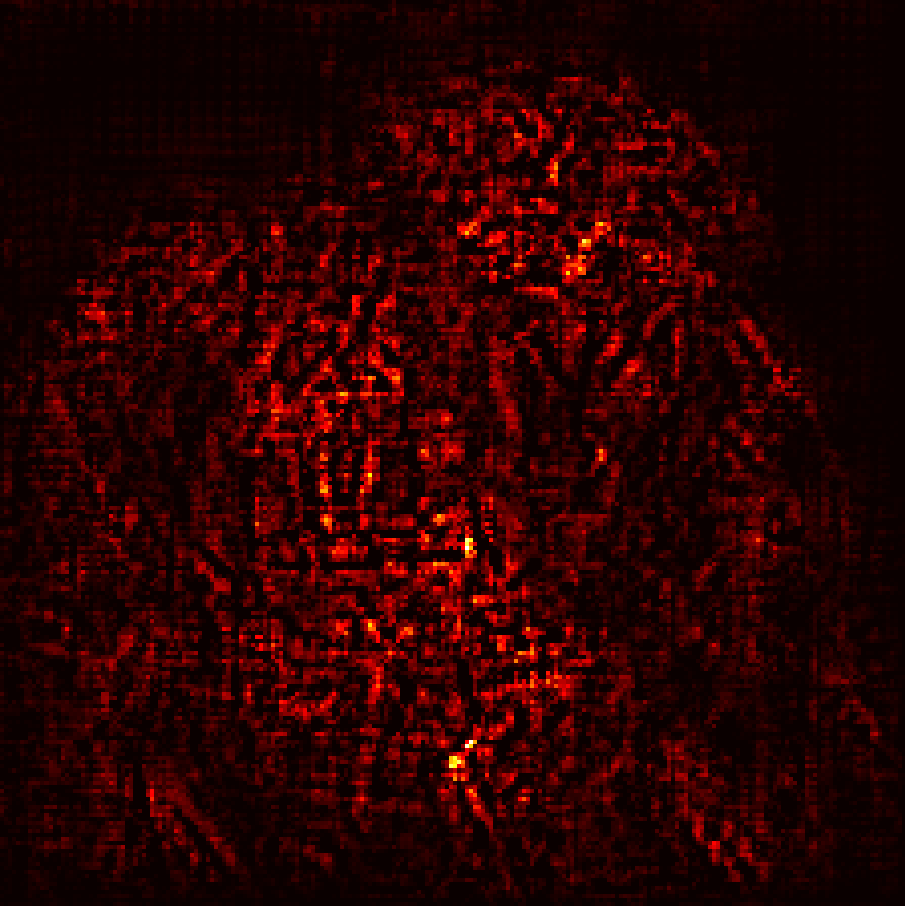
\includegraphics[width=\linewidth]{../visualizations/examples/imagenette/resnet18/negative_saliency_map/8.png}
        \caption{negative}
    \end{subfigure}
    \hfill
    \begin{subfigure}{0.14\textwidth}
        \centering
        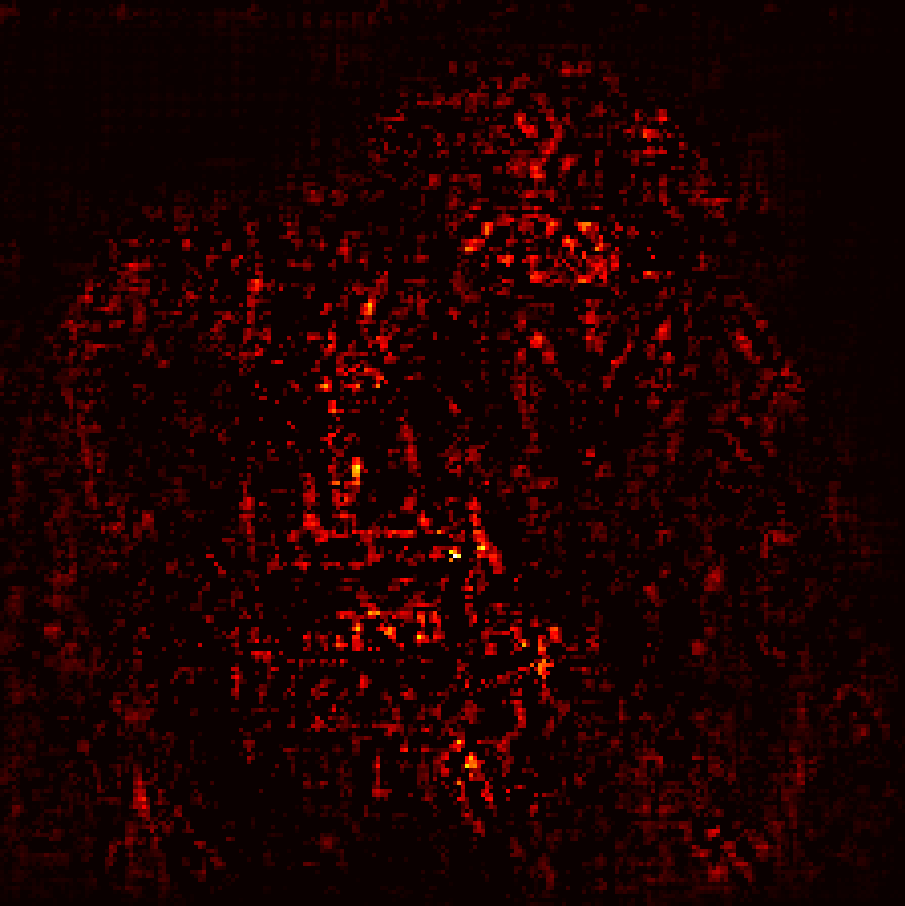
\includegraphics[width=\linewidth]{../visualizations/examples/imagenette/resnet18/active_saliency_map/8.png}
        \caption{active}
    \end{subfigure}
    \hfill
    \begin{subfigure}{0.14\textwidth}
        \centering
        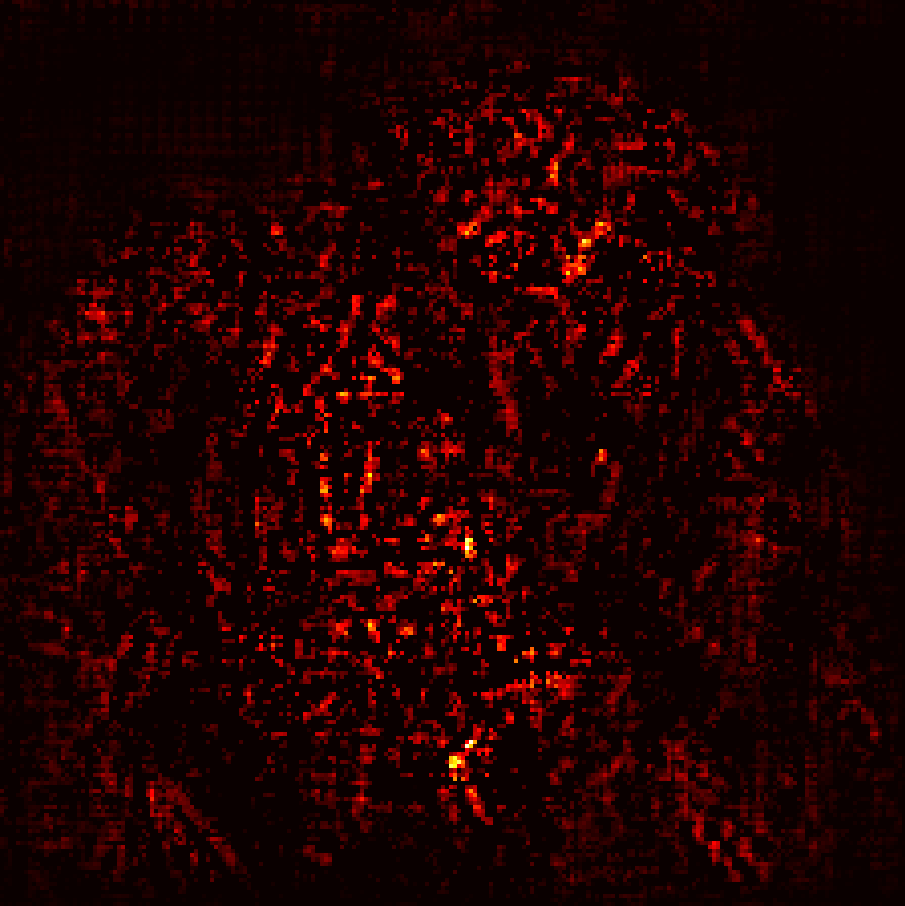
\includegraphics[width=\linewidth]{../visualizations/examples/imagenette/resnet18/inactive_saliency_map/8.png}
        \caption{inactive}
    \end{subfigure}
    \caption{Comparison Saliency Maps Resnet18 Imagenette}
    \label{fig: comparison saliency maps resnet18 imagenette}
\end{figure}

Following the same approach that can be found in the literature of Saliency Maps, first the techniques will be visually evaluated. In several papers, as in \cite{simonyanDeepConvolutionalNetworks2014a}, \cite{springenbergStrivingSimplicityAll2015}, \cite{smilkovSmoothGradRemovingNoise} or \cite{sundararajanAxiomaticAttributionDeep2017}, the different techniques were compared based on a visual inspection. 

One trend in the mentioned article is to just show some examples of the visualization to make the comparison. However, in none of them is explained how these examples are obtained. Therefore, it could be the case that the visualization is better for a certain class or example. To solve this problem in this paper a correct example for each class from the test is selected. These images are shown in Appendix~\ref{sec:signed saliency map examples}. Here, two examples can be observed in Figure~\ref{fig: comparison saliency maps cnn cifar10} and Figure~\ref{fig: comparison saliency maps resnet18 imagenette}.

From the comparison it can be appreciated that the proposed techniques reduce the noise of the original Saliency Maps, producing sharper visualization. The shape of the objects that the neural network is classifying are is clearer and there is a higher level of detail.

\subsection{Quantitative Evaluation}

\begin{figure}
    \centering
    \begin{subfigure}{0.49\linewidth}
        \centering
        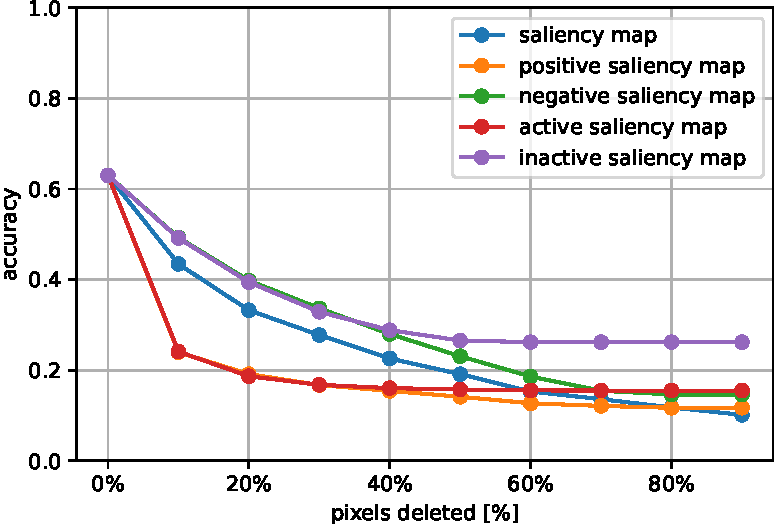
\includegraphics[width=\linewidth]{../visualizations/benchmarks/black_deletion/cifar10_cnn.pdf}
        \caption{Cifar10 CNN}
    \end{subfigure}
    \hfill
    \begin{subfigure}{0.49\linewidth}
        \centering
        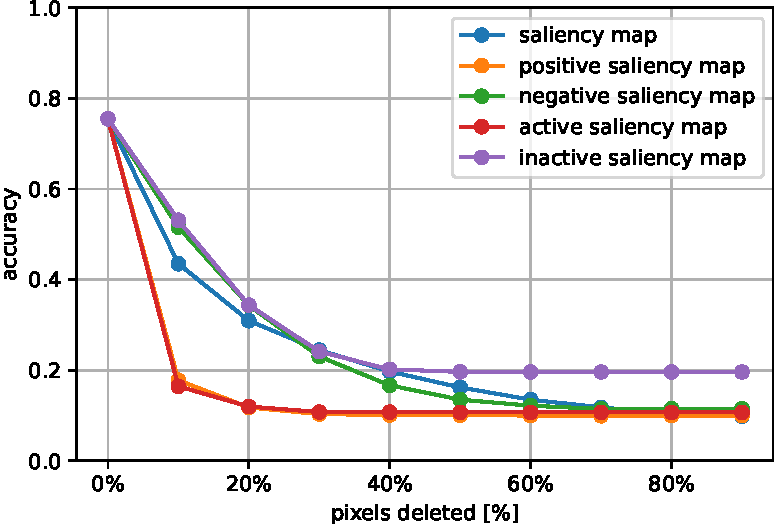
\includegraphics[width=\linewidth]{../visualizations/benchmarks/black_deletion/cifar10_resnet18.pdf}
        \caption{Cifar10 Resnet18}
    \end{subfigure}\\
    \hfill
    \begin{subfigure}{0.49\textwidth}
        \centering
        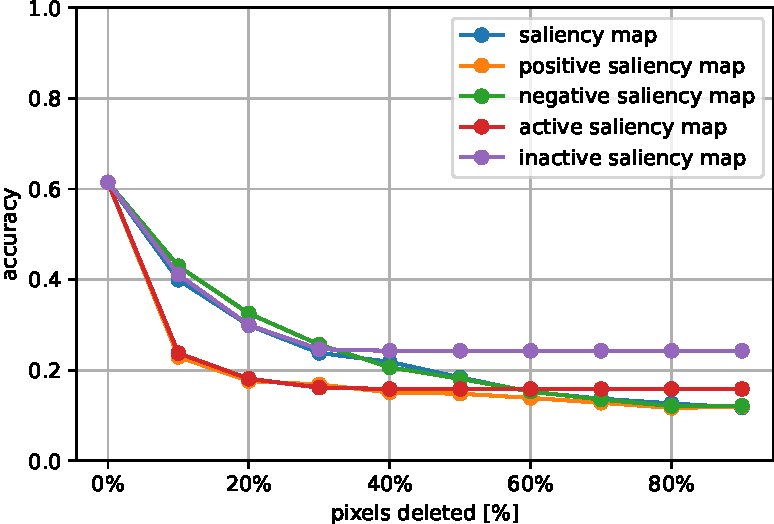
\includegraphics[width=\linewidth]{../visualizations/benchmarks/black_deletion/imagenette_cnn.pdf}
        \caption{Imagenette CNN}
    \end{subfigure}
    \hfill
    \begin{subfigure}{0.49\textwidth}
        \centering
        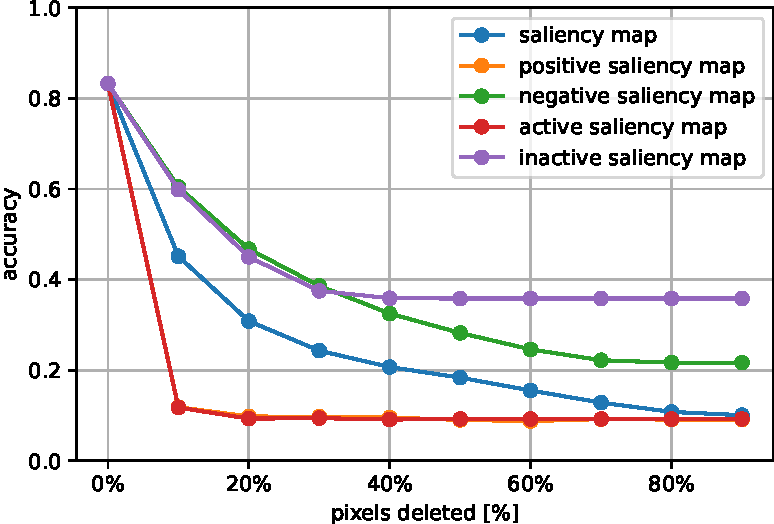
\includegraphics[width=\linewidth]{../visualizations/benchmarks/black_deletion/imagenette_resnet18.pdf}
        \caption{Imagenette Renset18}
    \end{subfigure}
    \caption{Black-Deletion Benchmark}
    \label{fig: black-deletion benchmark}
\end{figure}

\begin{figure}
    \centering
    \begin{subfigure}{0.49\linewidth}
        \centering
        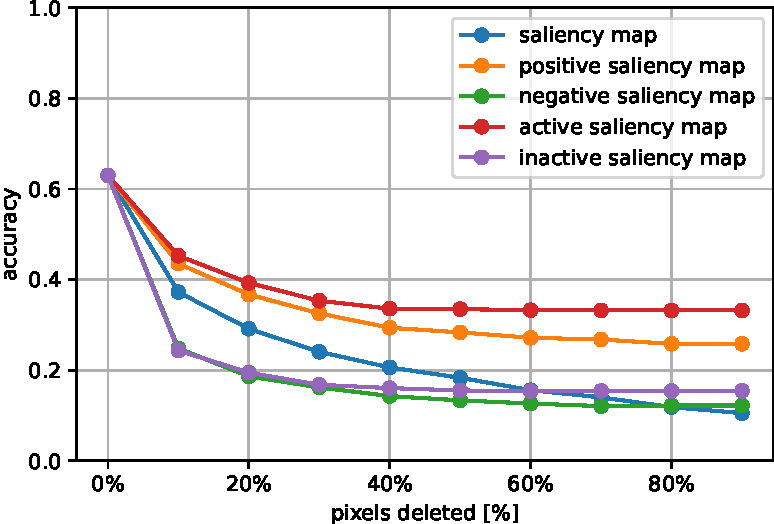
\includegraphics[width=\linewidth]{../visualizations/benchmarks/white_deletion/cifar10_cnn.pdf}
        \caption{Cifar10 CNN}
    \end{subfigure}
    \hfill
    \begin{subfigure}{0.49\linewidth}
        \centering
        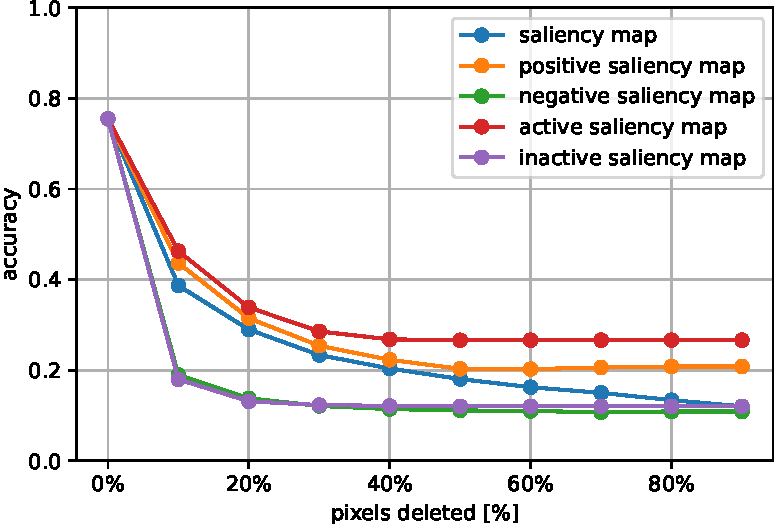
\includegraphics[width=\linewidth]{../visualizations/benchmarks/white_deletion/cifar10_resnet18.pdf}
        \caption{Cifar10 Resnet18}
    \end{subfigure}\\
    \hfill
    \begin{subfigure}{0.49\textwidth}
        \centering
        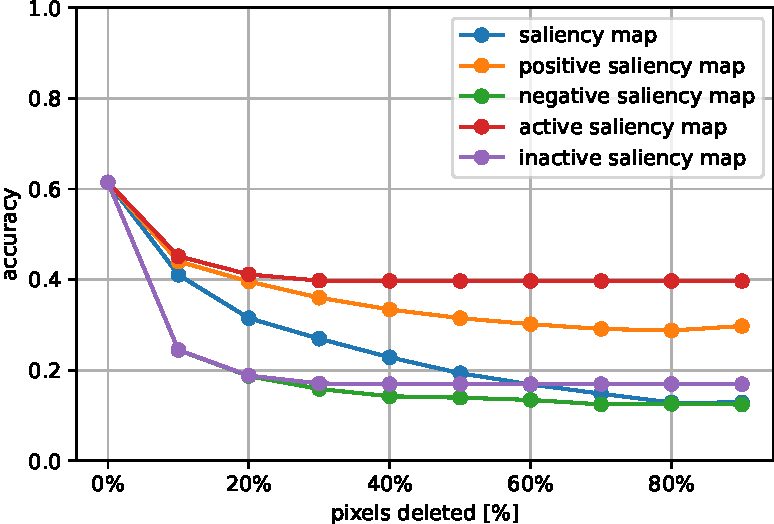
\includegraphics[width=\linewidth]{../visualizations/benchmarks/white_deletion/imagenette_cnn.pdf}
        \caption{Imagenette CNN}
    \end{subfigure}
    \hfill
    \begin{subfigure}{0.49\textwidth}
        \centering
        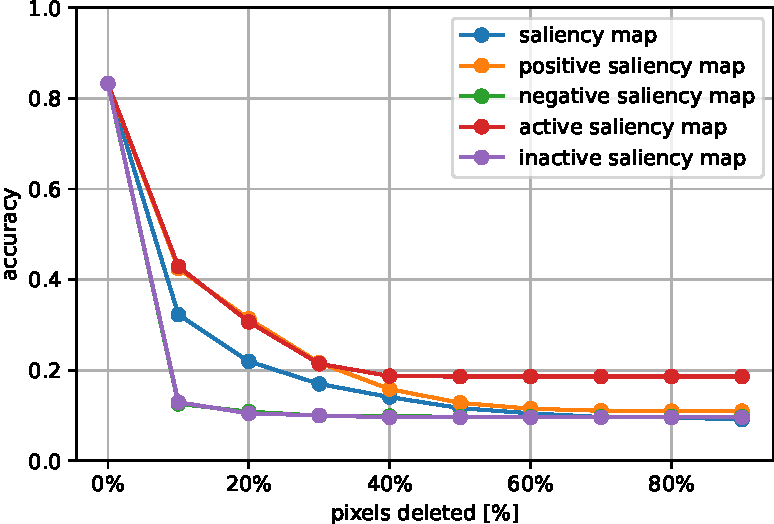
\includegraphics[width=\linewidth]{../visualizations/benchmarks/white_deletion/imagenette_resnet18.pdf}
        \caption{Imagenette Renset18}
    \end{subfigure}
    \caption{White-Deletion Benchmark}
    \label{fig: white-deletion benchmark}
\end{figure}

Even though historically the evaluation of Saliency Maps has been quanitative, there have been efforts to try to formulate metrics to measure the effectiveness of these techniques, as in 


\bibliographystyle{elsarticle-num} 
\bibliography{cas-refs}

\appendix

\section{Signed Saliency Map Examples}
\label{sec:signed saliency map examples}
hey this is gonna be awesome

%% If you have bibdatabase file and want bibtex to generate the
%% bibitems, please use
%%


%% else use the following coding to input the bibitems directly in the
%% TeX file.

% \begin{thebibliography}{00}

% %% \bibitem{label}
% %% Text of bibliographic item

% \bibitem{}

% \end{thebibliography}
\end{document}
\endinput
%%
%% End of file `elsarticle-template-num.tex'.
